\documentclass{article}
\usepackage[utf8]{inputenc}
\usepackage{geometry}
 \geometry{
 a4paper,
 total={170mm,257mm},
 left=20mm,
 top=20mm,
 }
 \usepackage{graphicx}
 \usepackage{titling}
\usepackage{mathptmx}
\usepackage{amsmath, amsthm, amssymb, calrsfs, wasysym, verbatim, bbm, color, graphics}
\usepackage{float}
\usepackage{longtable}
\usepackage{rotating}
\usepackage{adjustbox}
\usepackage{booktabs}
\usepackage{caption}
\usepackage[english]{babel}
\usepackage[table]{xcolor}
\usepackage{multicol}
\usepackage{hyperref}
\usepackage{amsmath}
\usepackage{listings}
\usepackage{pythonhighlight}
\lstnewenvironment{Python}[1][]{\lstset{style=mypython, frame=none, #1}}{}
 

 \title{Data and Information Quality Project
}
\author{Sofia Martellozzo}
\date{January 2023}
 
 \usepackage{fancyhdr}
\fancypagestyle{plain}{%  the preset of fancyhdr 
    \fancyhf{} % clear all header and footer fields
    \fancyfoot[R]{
\includegraphics[width=2cm]{logo_polimi.png}}
    \fancyfoot[L]{\thedate}
    \fancyhead[L]{DQ Project}
    \fancyhead[R]{\theauthor}
}
\makeatletter
\def\@maketitle{%
  \newpage
  \null
  \vskip 1em%
  \begin{center}%
  \let \footnote \thanks
    {\LARGE \@title \par}%
    \vskip 1em%
    %{\large \@date}%
  \end{center}%
  \par
  \vskip 1em}
\makeatother

\usepackage{lipsum}  
\usepackage{cmbright}

\begin{document}

\maketitle

\noindent\begin{tabular}{@{}ll}
    Student & \theauthor\\
     StudentID &  996215\\
     Student Personal Code & 10623060\\
      & \\
     Project ID & 18\\
     Assigned Dataset & \texttt{letter.csv}\\
     Assigned Task & Classification
\end{tabular}

\section*{Introduction}
In this project is faced a Classification problem , with two different Machine Learning algorithm, after an imputation of data on the datasets provided, where it encounter NaN values, with two different techniques.\\\\
The dataset is composed of 2001 samples and 17 labels: 'x-box', 'y-box', 'width', 'high’,  'onpix', 'x-bar', 'y-bar', 'x2bar', 'y2bar', 'xybar', 'x2ybr', 'xy2br', 'x-ege', 'xegvy', 'y-ege', 'yegvx' and 'letter' , that is the target  to predict. The values of the different labels are almost all around 0 and 15, while the target are 26 different letters: 'L', 'F', 'Z', 'T', 'U', 'H', 'Y', 'B', 'R', 'O', 'X', 'S', 'M', 'P', 'K', 'Q', 'V', 'C', ‘W’,  'N', 'G', 'J', 'E', 'A', 'I', 'D' .
\section{Setup choices}
\subsection{Chosen ML algorithm}
Supervised learning learns a function to make prediction of a defined label based on the input data. It can be either classifying data into a category (classification problem) or forecasting an outcome (regression algorithms).\\
Classification model identifies which category an object belongs to whereas regression model predicts a continuous output. Sometimes there is an ambiguous line between classification algorithms and regression algorithms.\\
Many algorithms can be used for both classification and regression, and classification is just regression model with a threshold applied. When the number is higher than the threshold it is classified as true while lower classified as false. \\\\
Here follows the description of the two ML algorithm selected to solve the Classification problem on the {\texttt letter} dataset.
\subsubsection*{Support Vector Classifier (SVC)}
\begin{multicols}{2}
\begin{figure}[H]
        \begin{center}
        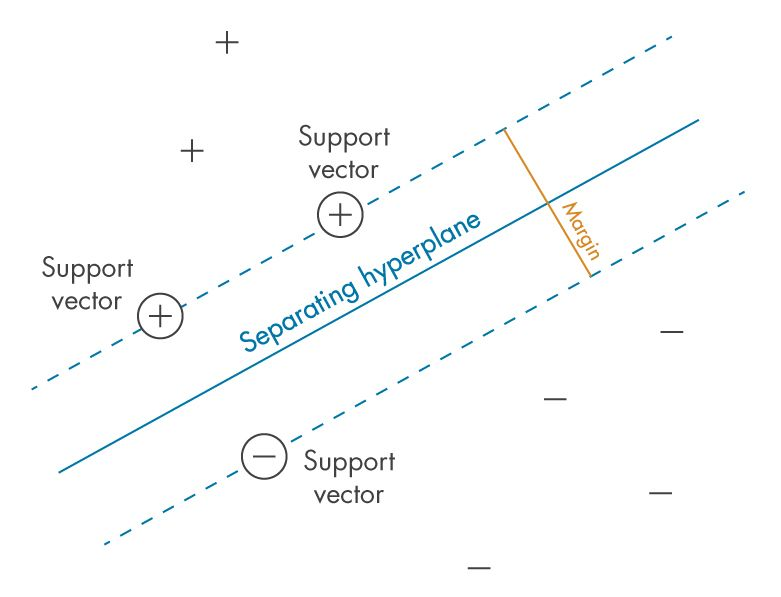
\includegraphics[width=0.4\textwidth]{SVC.jpeg}
        \end{center}
    \end{figure} 
    \columnbreak
\columnbreak
Support Vector Classifier (SVC) is developed based on Support Vector Machine (SVM): a type of deep learning algorithm, builds a learning model that assigns new examples to one group or another. By these functions, SVMs are called a non-probabilistic, binary linear classifier. SVM finds the best way to classify the data based on the position in relation to a border between positive class and negative class. This border is known as the hyperplane which maximize the distance between data points from different classes.
\end{multicols}
\begin{center}
How is implemented in python:
\begin{Python}
from sklearn.svm import SVC
svc = SVC()
svc.fit(X_train, y_train)
y_pred = svc.predict(X_test)
\end{Python}
\end{center}


\newpage
\subsubsection*{Decision Tree}
\begin{multicols}{2}
\begin{figure}[H]
        \begin{center}
        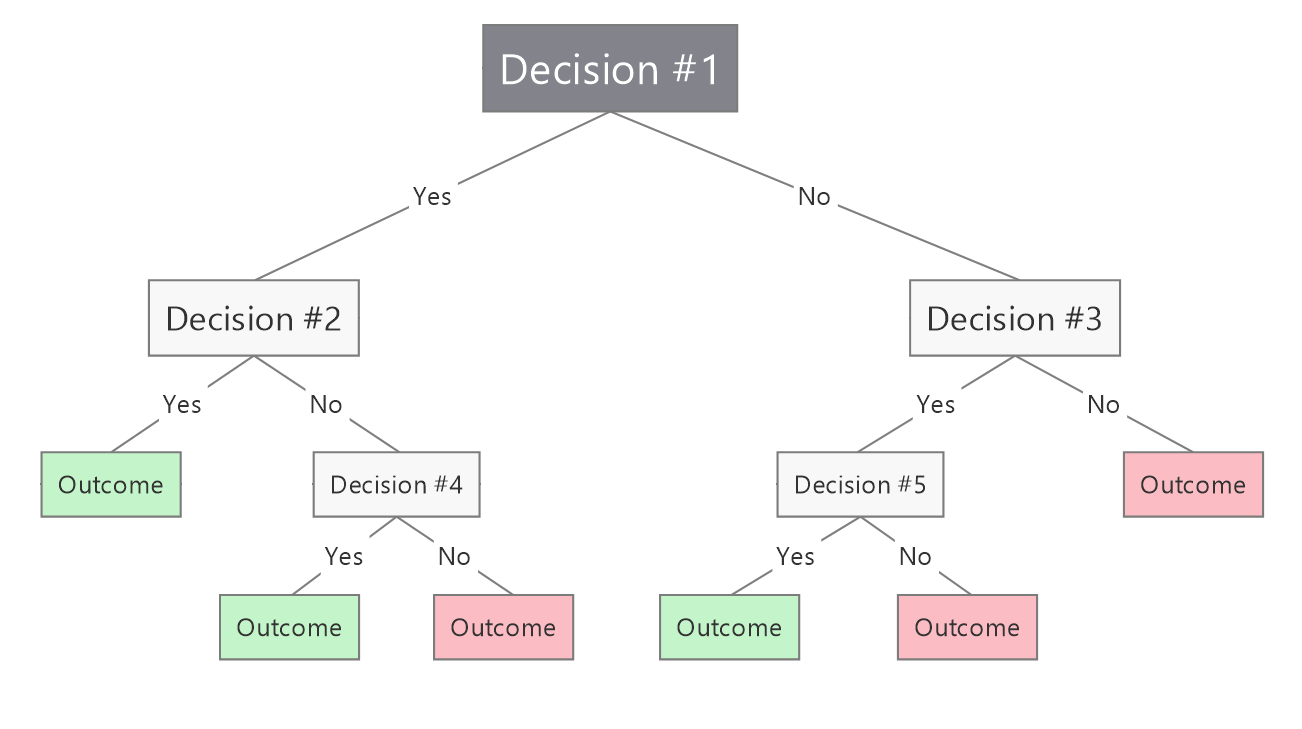
\includegraphics[width=0.4\textwidth]{DecTree.png}
        \end{center}
    \end{figure} 
    \columnbreak
\columnbreak
Descr...\\

\end{multicols}
How is implemented in python:
\begin{Python}
from sklearn.tree import DecisionTreeClassifier
dtc = DecisionTreeClassifier()
dtc.fit(X_train, y_train)
y_pred = dtc.predict(X_test)
\end{Python}





\subsection{Chosen ML performance evaluation metrics}
\subsection{Imputation techniques selected}

\section{Pipeline implementation}
description of the steps you performed

\section{Results}
description of the main result obtained\\
b.	ML performance comparison between the imputation techniques you have implemented



\end{document}
